\begin{frame}{Calcul de pertinence des concepts}
Trois mesures de pondération : \textsc{TF-IDF}, \textsc{BM25} et \textsc{BERT}.
    \footnotesize
\begin{table}[]
\begin{tabular}{|l|cccc|}
\hline
\multicolumn{1}{|c|}{\multirow{}{}{Terme}} & \multicolumn{4}{c|}{\cellcolor{gray!10!white}{ Corpus \textrm{Autres}}}                              \\ \cline{2-5} 
\multicolumn{1}{|c|}{}                       & \multicolumn{1}{c}{{Fréquence}} & \multicolumn{1}{c}{{TF-IDF}} & \multicolumn{1}{c}{{BM25}}  & {BERT} \\ \hline
{Arthrite déformante} &
  \multicolumn{1}{|r|}{{24}} &
  \multicolumn{1}{|r|}{{0,02}} &
  \multicolumn{1}{|r|}{{0,50}} &
  {0,40} \\ \hline
{Ataxie locomotrice} &
  \multicolumn{1}{|r|}{{169}} &
  \multicolumn{1}{|r|}{{0,08}} &
  \multicolumn{1}{|r|}{{0,25}} &
  {0,39} \\ \hline
{Atrophie musculaire} &
  \multicolumn{1}{|r|}{{1465}} &
  \multicolumn{1}{|r|}{{0,43}} &
  \multicolumn{1}{|r|}{{0,15}} &
  {0,42} \\ \hline
{Atrophie progressive} &
  \multicolumn{1}{|r|}{{22}} &
  \multicolumn{1}{|r|}{{0,02}} &
  \multicolumn{1}{|r|}{{0,53}} &
  {0,39} \\ \hline
{Catalepsie} &
  \multicolumn{1}{|r|}{{975}} &
  \multicolumn{1}{|r|}{{0,28}} &
  \multicolumn{1}{|r|}{{0,15}} &
  {0,39} \\ \hline
{Épilepsie} &
  \multicolumn{1}{|r|}{{577}} &
  \multicolumn{1}{|r|}{{0,12}} &
  \multicolumn{1}{|r|}{{0,10}} &
  {0,41} \\ \hline
{Hystérie} &
  \multicolumn{1}{|r|}{{4934}} &
  \multicolumn{1}{|r|}{{0,45}} &
  \multicolumn{1}{|r|}{{0,05}} &
  {0,41} \\ \hline
{Langue} &
  \multicolumn{1}{|r|}{{3591}} &
  \multicolumn{1}{|r|}{{0,11}} &
  \multicolumn{1}{|r|}{{0,02}} &
  {0,41} \\ \hline
{Maladie de Parkinson} &
  \multicolumn{1}{|r|}{{130}} &
  \multicolumn{1}{|r|}{{0,09}} &
  \multicolumn{1}{|r|}{{0,35}} &
  {0,37} \\ \hline
{Paralysie bulbaire} &
  \multicolumn{1}{|r|}{{93}} &
  \multicolumn{1}{|r|}{{0,09}} &
  \multicolumn{1}{|r|}{{0,52}} &
  {0,40} \\ \hline
{Paralysie rhumatismale} &
  \multicolumn{1}{|r|}{{14}} &
  \multicolumn{1}{|r|}{{0,02}} &
  \multicolumn{1}{|r|}{{0,68}} &
  {\cellcolor{green!30!white}{\textcolor{purple}{\textbf{0,44}}}} \\ \hline
{Sclérose latérale} &
  \multicolumn{1}{|r|}{{127}} &
  \multicolumn{1}{|r|}{{0,09}} &
  \multicolumn{1}{|r|}{{0,37}} &
  {0,41} \\ \hline
{Sclérose en plaque disséminées} &
  \multicolumn{1}{|r|}{{12}} &
  \multicolumn{1}{|r|}{{0,02}} &
  \multicolumn{1}{|r|}{\cellcolor{green!30!white}{\textcolor{purple}{\textbf{0,83}}}} &
  {0,40} \\ \hline
{Somnambulisme} &
  \multicolumn{1}{|r|}{{3410}} &
  \multicolumn{1}{|r|}{\cellcolor{green!30!white}{\textcolor{purple}{\textbf{1}}}} &
  \multicolumn{1}{|r|}{{0,15}} &
  {0,43} \\ \hline
\end{tabular}
\caption{Pertinence des concepts sous forme des scores TF-IDF, BM25 et BERT, corpus \textrm{Autres}.}
\end{table}
\end{frame} 

\begin{frame}{Intensification du discours
de Charcot dans le corpus \textrm{Autres}}
Le terme le plus impactant dans le réseau de Charcot selon \textsc{BM25} :\\
\textit{sclérose en plaque disséminées} ? (pertinence : 83\%)
\begin{figure}[!h]
    \centering
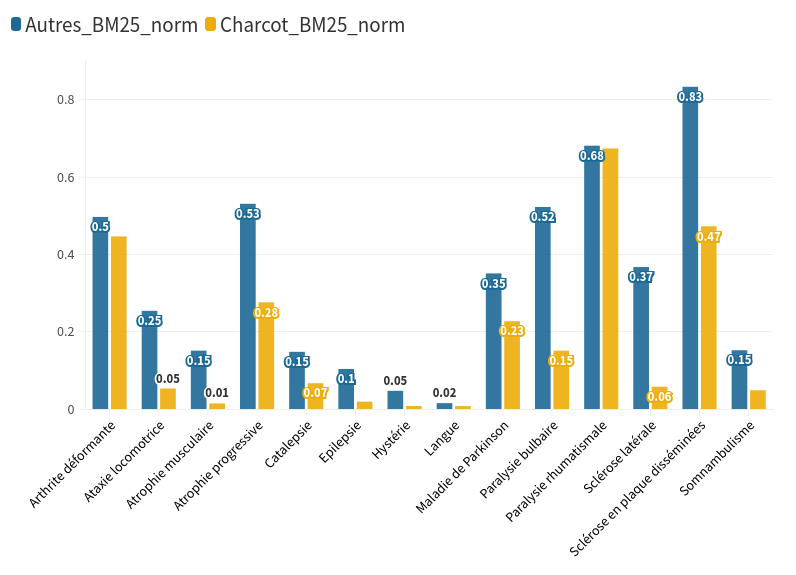
\includegraphics[width=80mm,scale=0.5]{pic/Charcot_Autres_250523.png}
    \caption{Pertinence des concepts dans les deux corpus (BM25).}
    \label{fig:my_label}
\end{figure}
\end{frame}

\begin{frame}{Types de concepts extraits avec \textsc{BERT}}
    \begin{itemize}
        \item plongements lexicaux et des
mécanismes d’attention
        \item modèle \texttt{bert-base-multilingual-cased}
    \end{itemize}
    \begin{flushright}
    {(\small \cite{vaswani2017})}
    \end{flushright}

\begin{table}[]
\begin{tabular}{|ll|ll|}
\hline
\multicolumn{2}{|c|}{\cellcolor[HTML]{EFEFEF}Corpus \textrm{Charcot}} & \multicolumn{2}{c|}{\cellcolor[HTML]{EFEFEF}Corpus \textrm{Autres}}     \\ \hline
\multicolumn{1}{|l|}{diplopie}                & 0,92 & \multicolumn{1}{l|}{préambule}       & 0,47      \\
\multicolumn{1}{|l|}{myélite partielle}       & 0,91 & \multicolumn{1}{l|}{délire}          & 0,47      \\
\multicolumn{1}{|l|}{état de mal épileptique} & 0,91 & \multicolumn{1}{l|}{miracle}         & 0,47      \\
\multicolumn{1}{|l|}{paralysie labio-glosso-laryngée} & 0,91 & \multicolumn{1}{l|}{cicatrices vicieuses} & 0,46 \\ \hline
\multicolumn{2}{|c|}{\cellcolor[HTML]{E1FFE1}\textsc{pathologies}}     & \multicolumn{2}{c|}{\cellcolor[HTML]{FFDFDD}\textsc{notions abstraites}} \\ \hline 
\end{tabular}
\end{table}
\end{frame}

\begin{frame}{Extraction des phrases-clés : méthode \texttt{keybert}}
\begin{enumerate}
\small
\item entrée : un document
\item tokénisation du document en phrases-clés candidates (PCC)
\item génération des plongements du doc. et des PCC par un modèle de langage
\item calcul de la similarité cosinus entre le document et les PC
\end{enumerate}
\begin{figure}
    \centering
    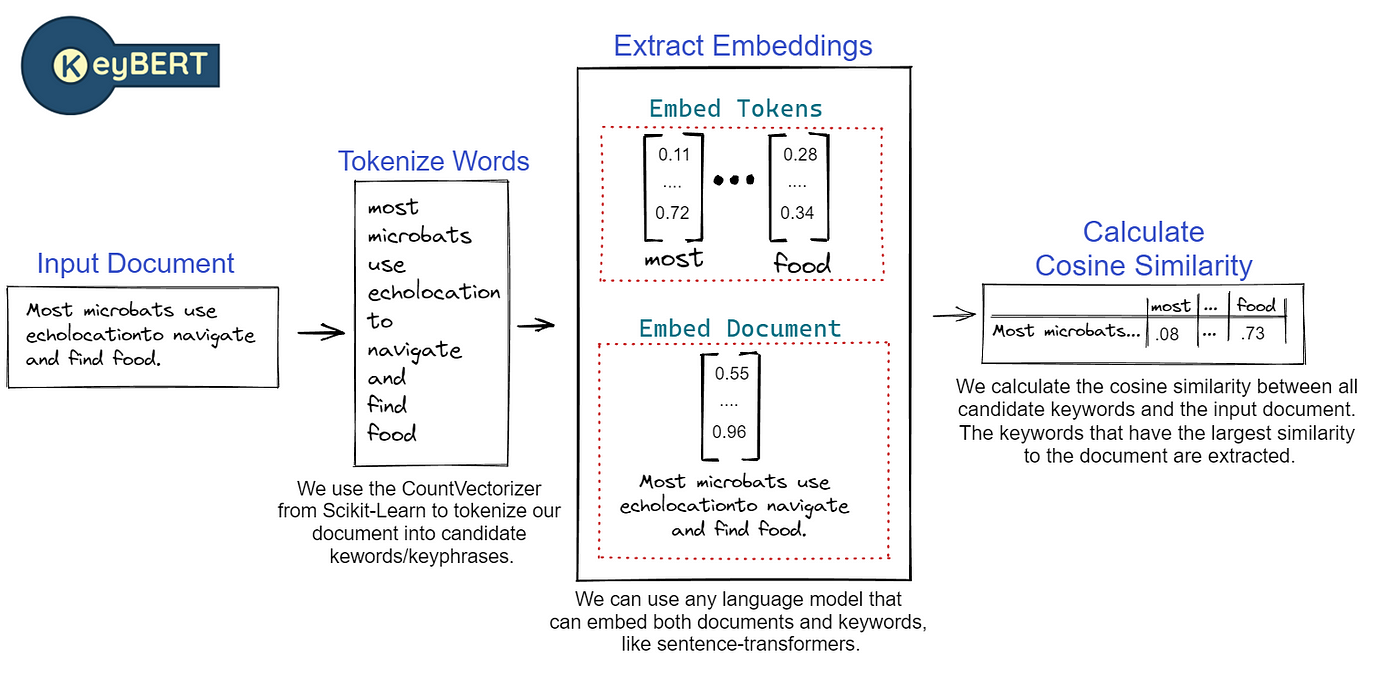
\includegraphics[width=80mm,scale=0.5]{pic/keybert.png}
    \caption{\textit{Pipeline} de la librairie \texttt{keybert} \citep{grootendorst2020keybert}.}
    \label{fig:enter-label}
\end{figure}
\end{frame}

\begin{frame}{Limitations de \texttt{keybert}}
\danger{} manque de diversification des résultats + (non-)grammaticalité\\
{\small 2 termes communs : \og{}articulations de épaule\fg{}, \og{}paralysie faciale périphérique\fg{}}
    \begin{figure}[!ht]
        \centering
        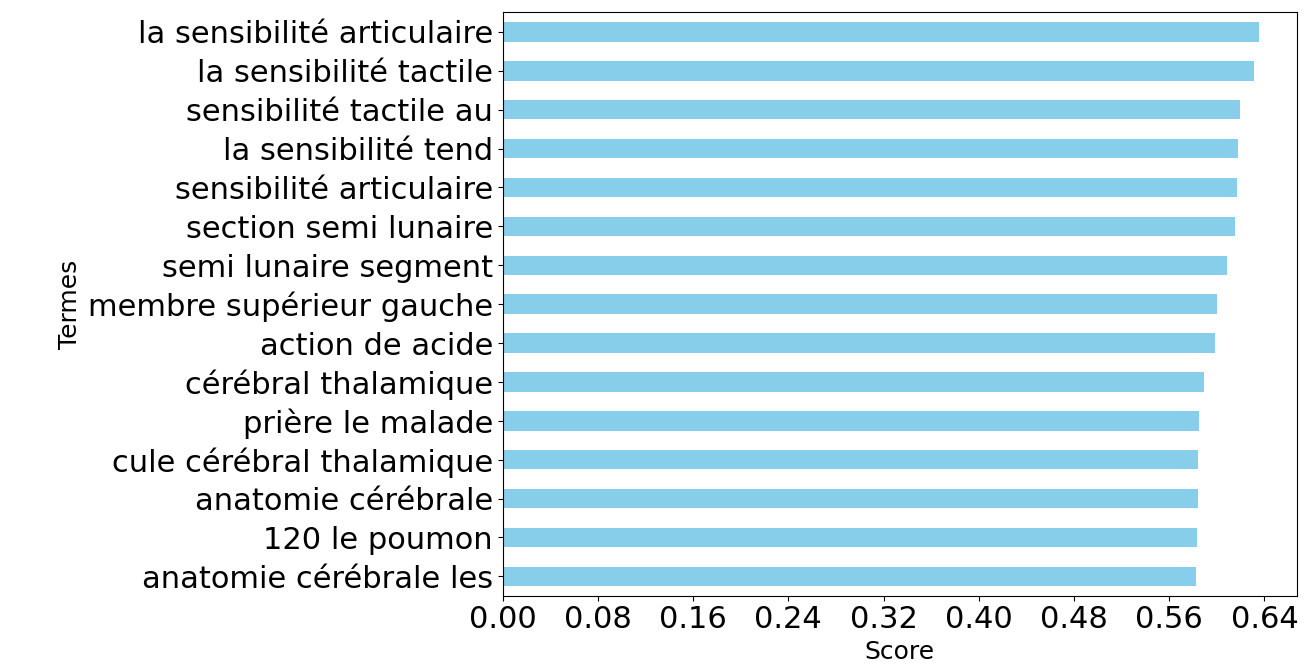
\includegraphics[width=100mm,scale=0.5]{pic/termes_keybert_autres.png}
        \caption{Répartition des 15 termes les plus pertinents dans le corpus \textrm{Autres} selon \texttt{keybert}.}
        \label{fig:enter-label}
    \end{figure}
\end{frame}

%\begin{frame}{Phrases-clés \textit{hapax} partagés dans les deux corpus selon \texttt{keybert}}
%Les seuls termes partagés avec le corpus Charcot : 
%%\begin{itemize}
%%\item articulations de [\textit{sic}] épaule
%%\item paralysie faciale périphérique
%%\end{itemize}
%    \begin{figure}[!ht]
%        \centering
%        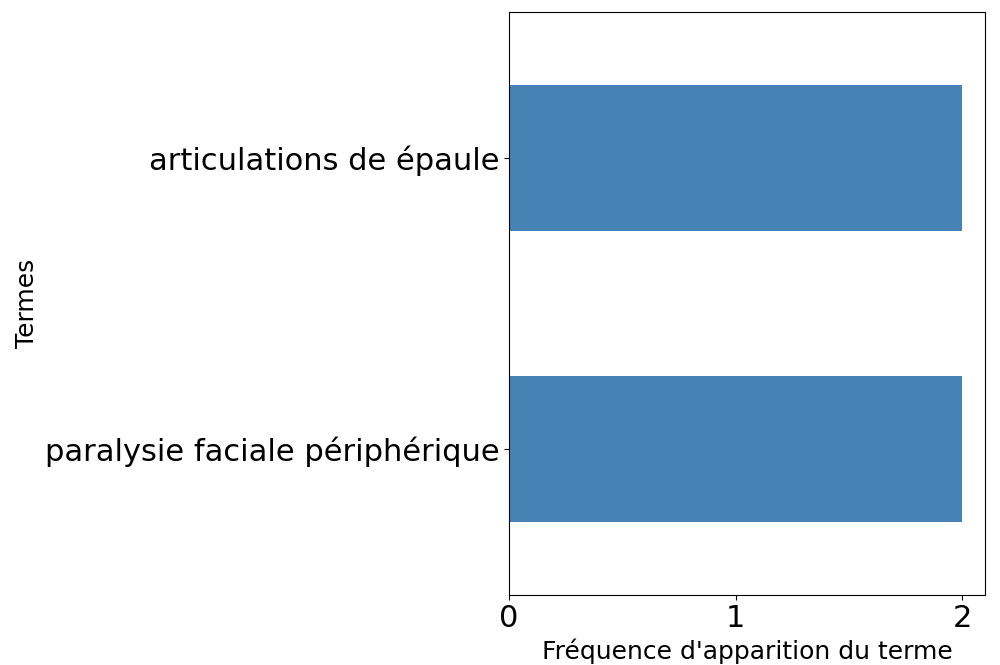
\includegraphics[width=90mm,scale=0.5]{pic/termes_partages_keybert.png}
%        \caption{Répartition des termes les plus pertinents dans les deux corpus selon \texttt{keybert}.}
%        \label{fig:enter-label}
%    \end{figure}
%\end{frame}
\begin{frame}{Extraction des phrases-clés : méthode \textit{PatternRank}\\
\quad \quad \quad\ \quad \quad \quad \quad \quad \quad \quad \ \ \ \ \ \small{Librairie \texttt{keyphrase-vectorizers}}}
%\begin{itemize}
%\item extraction des phrases-clés non-supervisée
%\item exploite des modèles de langues pré-entraînés + parties du discours
%\end{itemize}
\begin{enumerate}
\small
\item entrée : un seul document texte tokenisé
\item étiquetage des tokens avec les balises du partie du discours (POS)
\item sélection des tokens selon le motif POS $\rightarrow$ phrases-clés candidates (PCC)
\item génération des plongements du doc. et des PCC par un modèle de langue
\item calcul des similarités cosinus entre ces deux types de plongements +  \\classement des PCC par ordre décroissant
\item extraction des \textit{N} PC les plus représentatives
\end{enumerate}
\begin{figure}
    \centering
    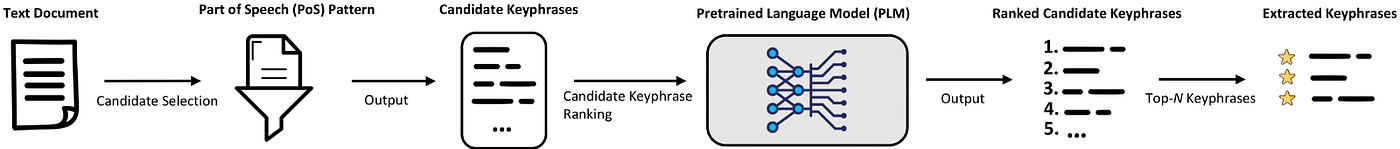
\includegraphics[width=110mm,scale=0.5]{pic/patternrank_workflow.png}
    \caption{\textit{Workflow} de la méthode \textit{PatternRank} \citep{schopf2022}.}
    \label{fig:enter-label}
\end{figure}
\notecite{schopf2022}
\end{frame}

%\begin{frame}{Termes partagés extraits avec \texttt{keyphrase-vectorizers}}
%    \begin{figure}[!ht]
%        \centering
%        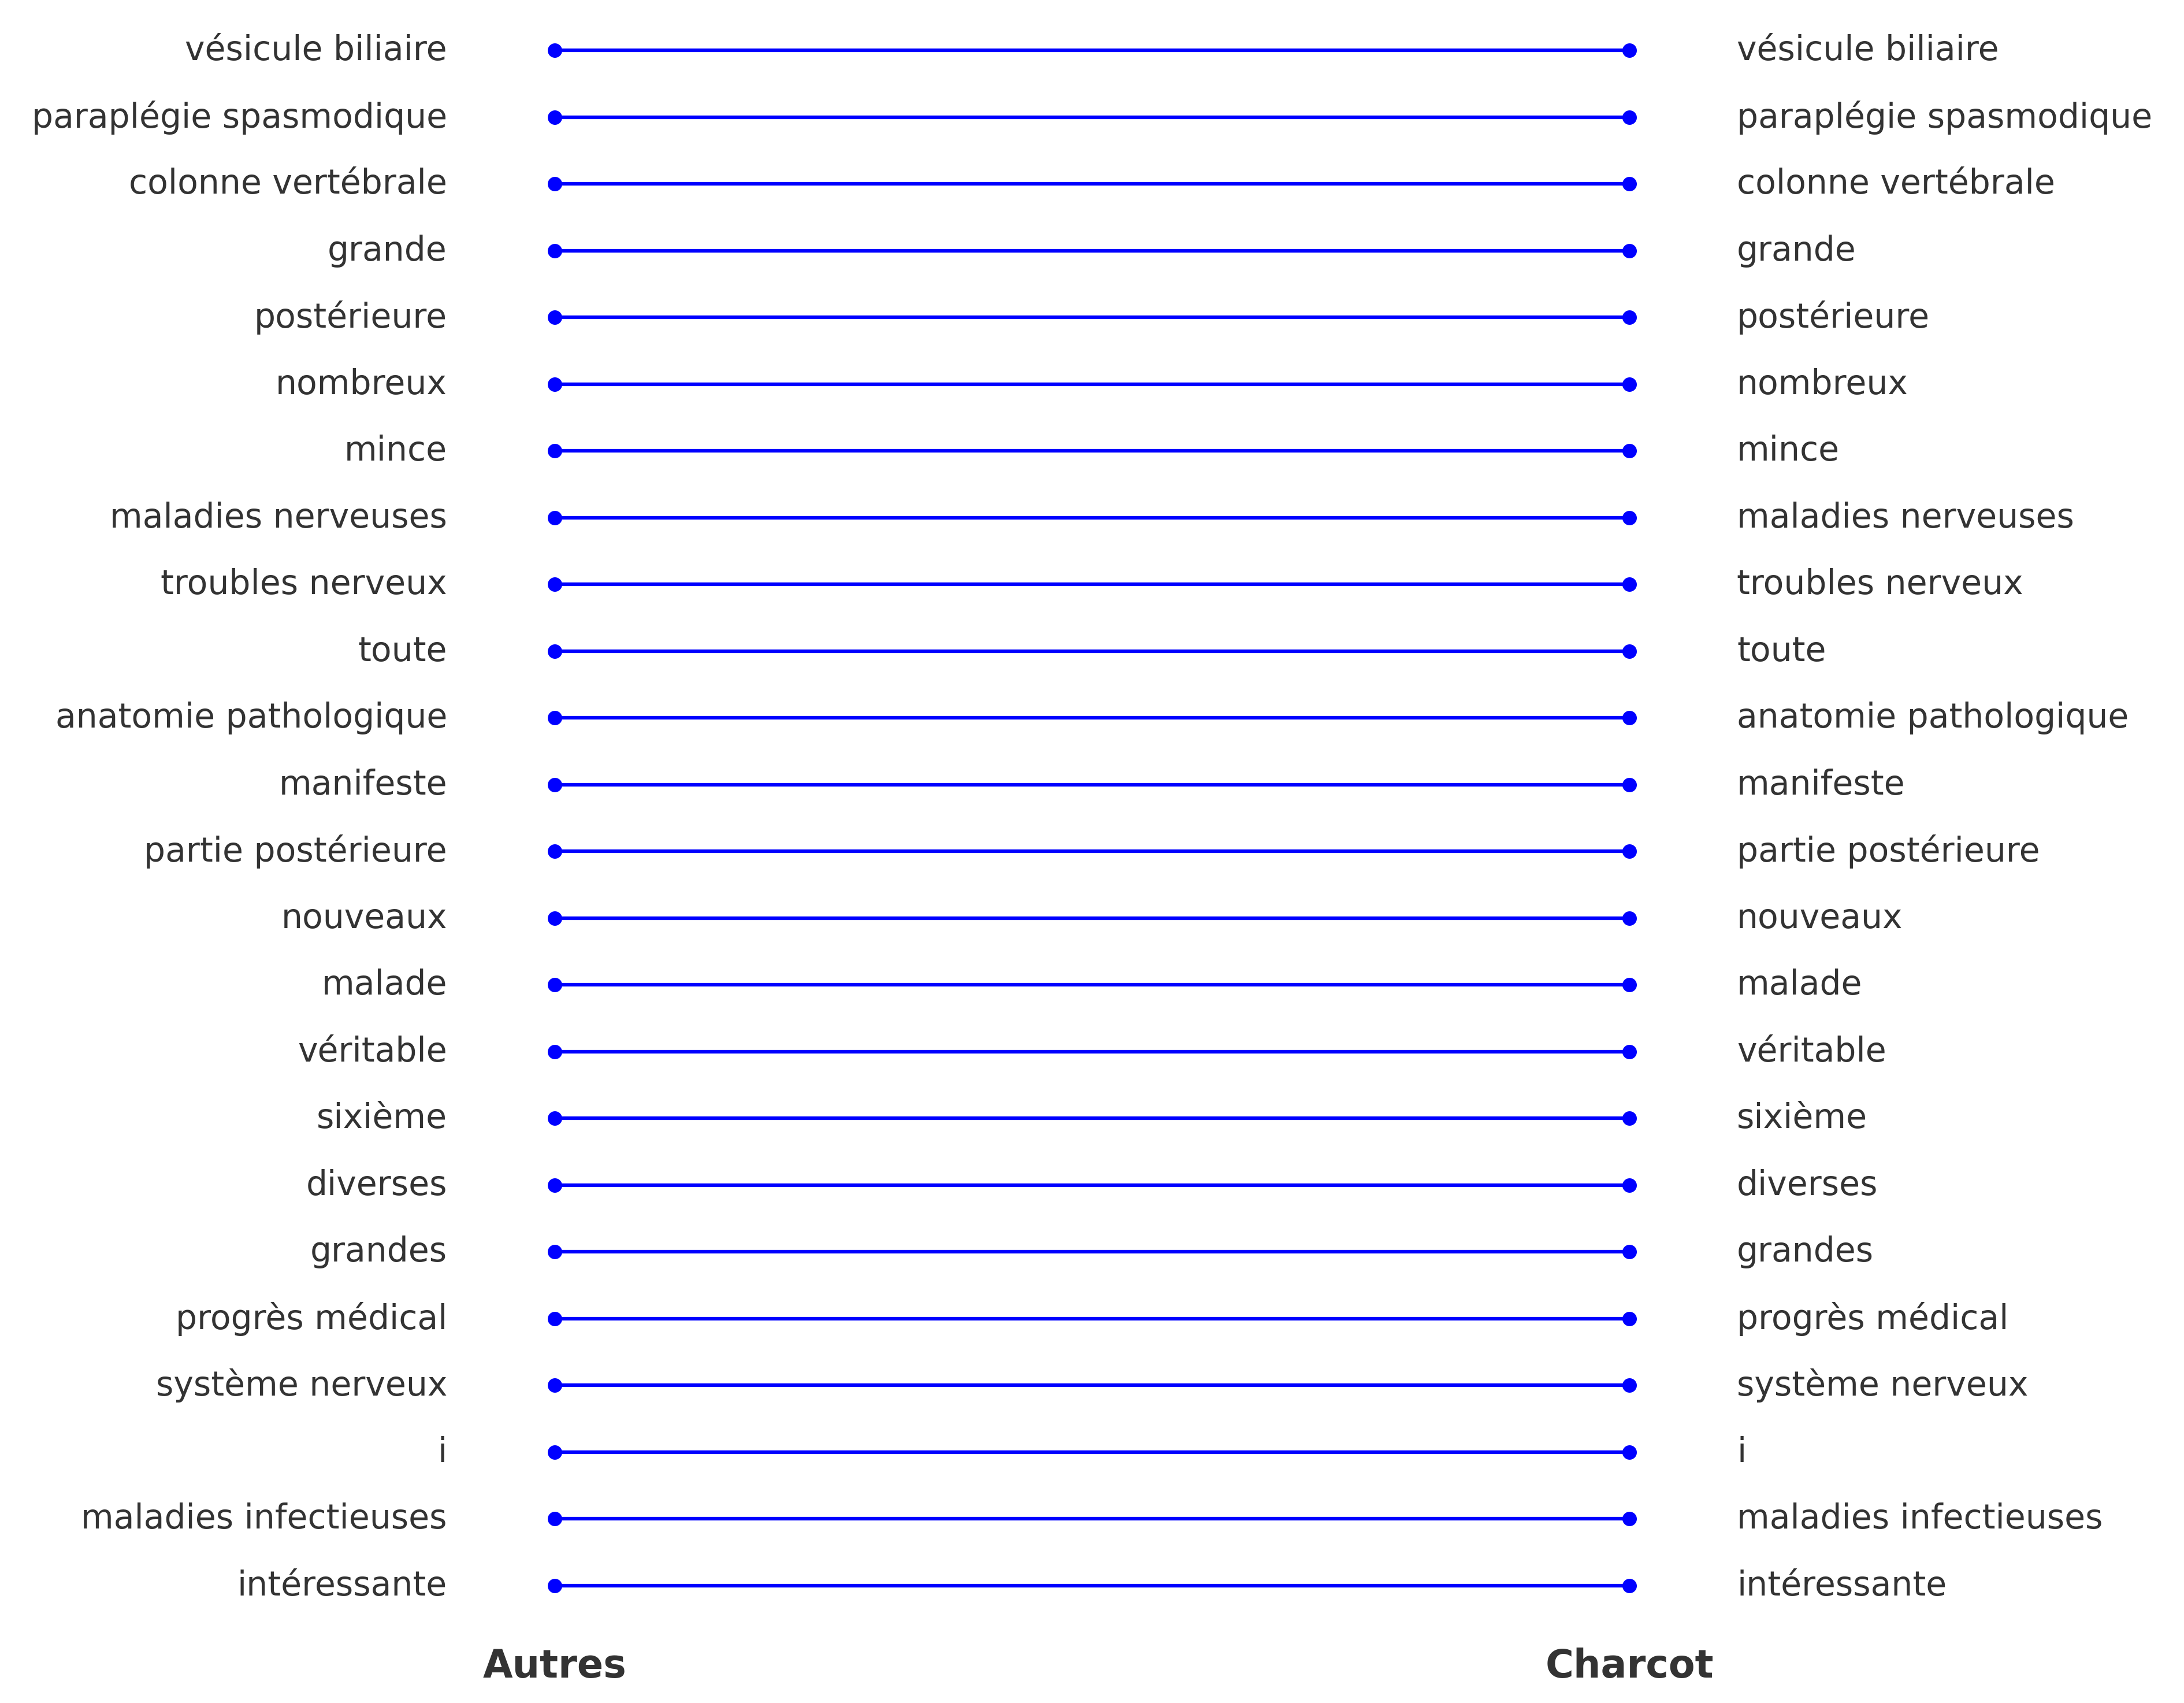
\includegraphics[width=85mm,scale=0.5]{pic/visualisation_termes_dupliques.png}
%        \caption{Les termes communs aux deux corpus selon \texttt{keyphrase-vectorizers}.}
%        \label{fig:enter-label}
%    \end{figure}
%\end{frame}

%\begin{frame}{Termes partagés | \texttt{keyphrase-vectorizers}}
%    \begin{figure}[!ht]
%        \centering
%        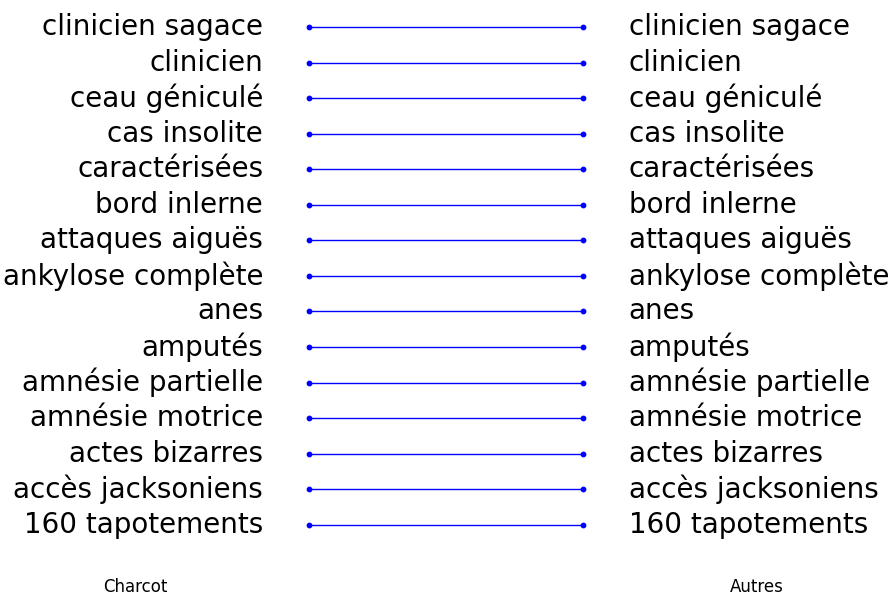
\includegraphics[width=100mm,scale=0.5]{pic/termes_partages_liens.png}
%        \caption{Les termes communs (fréq. = 1) aux deux corpus selon \texttt{keyphrase-vectorizers}.}
%        \label{fig:enter-label}
%    \end{figure}
%\end{frame}

\begin{frame}{Les termes partagés les plus fréquents | \texttt{keyphrase-vectorizers}}
    \begin{figure}[!ht]
        \centering
        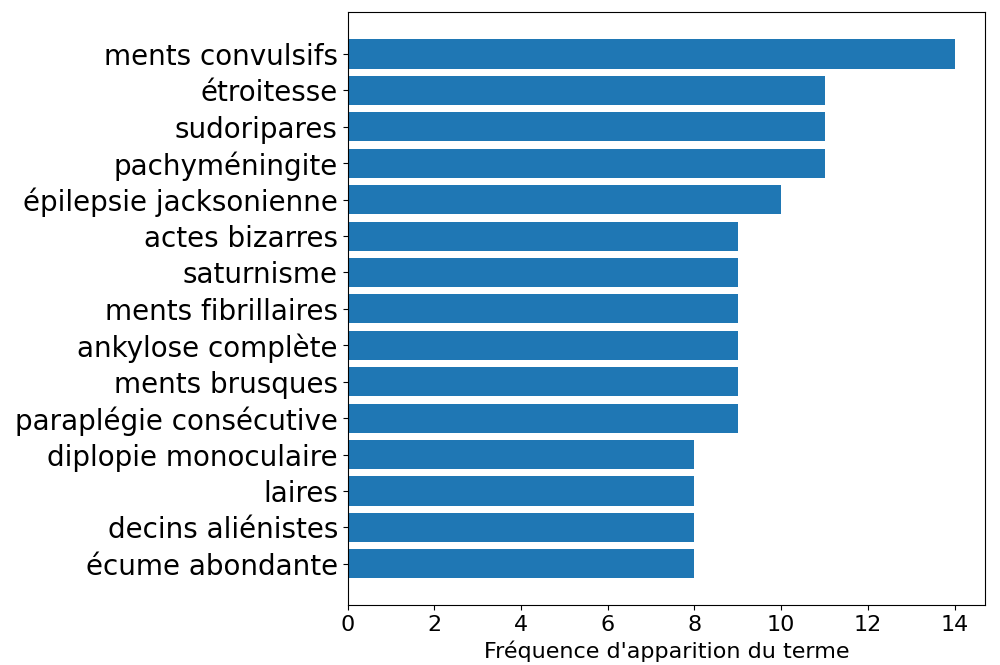
\includegraphics[width=100mm,scale=0.5]{pic/termes_partages.png}
        \caption{Les 15 termes les plus fréquents dans les deux corpus selon \texttt{keyphrase-vectorizers}.}
        \label{fig:enter-label}
    \end{figure}
\end{frame}